\documentclass[11pt]{article}

\usepackage{graphicx}
\usepackage{float}

% Margins
\topmargin=-0.45in
\evensidemargin=0in
\oddsidemargin=0in
\textwidth=6.5in
\textheight=9.0in
\headsep=0.25in

\title{CS 3600 Project Phase 3}
\author{Jake Gendreau, Michael Crapse}
\date{\today}

\begin{document}
\maketitle	

\begin{figure}[H]
    \centering
    
\includegraphics[width=0.5\textwidth]{../../icon.png}
\end{figure}

\tableofcontents
\newpage

\section{Project}
    StockUp is a social and financial app which is a combination of fantasy football and real-world investment.
    On StockUp, users will be able to join a team, invest in stocks, and earn money for their team.

\section{System Design}
    \subsection{Database}

    \begin{figure}[H]
        \centering
        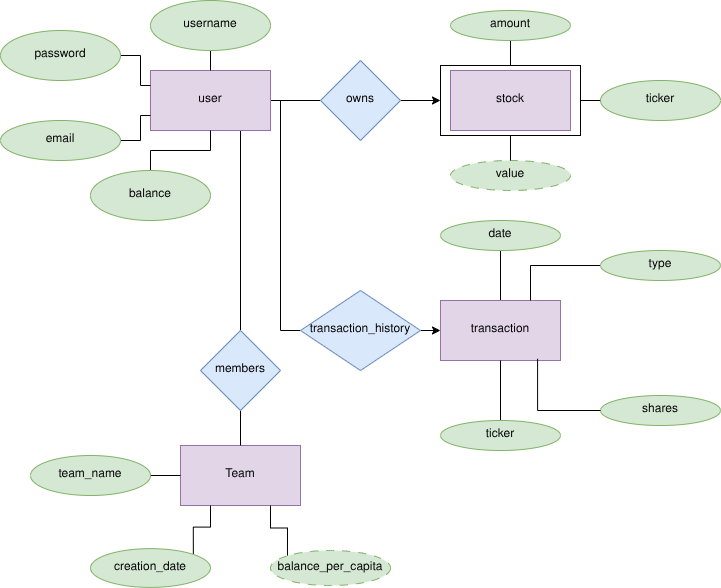
\includegraphics[width=0.7\linewidth]{image4.png}
        \caption{ER Diagram}
        \label{fig:image4}
    \end{figure}

    Django and SQLite3 are used to create and query the database.
    The tables are generated by Django with the models.py file.
    Any changes made to the database model are applied by executing the migrate command with manage.py.

    \subsection{Backend}
    The backend routes are routed by Django.
    All routes are implemented in the views.py file.
    The routing URLs are assigned in the urls.py file from implementations in the views.py file.

    \subsection{Frontend}
    The frontend is designed with HTML and Bootstrap templates generated with Django.
    Templates are stored in the templates directory with static resources from the static directory.
    Essentially, HTML files are stored in the templates directory and CSS/JS files are stored in the static directory for sharing.

    \subsection{Stock Predictor}
    The stock information is gained from the Yahoo Finance package, yfinance.
    The stock predictor model is implemented with XGBoost and stored as a file that is restored with the joblib package.
    The joblib package allows for the model to be trained once to reduce prediction times.

    A prediction may be obtained through a POST request sent to the invest route.
    The POST request body requires a ticker symbol and a sector.

\section{Functional Components}
    \subsection{Database}
    The database is fully implemented.

    \subsection{Backend}
    The core features of the backend are implemented with routes, database, and pages.

    \subsection{Frontend}
    User interface is complete and the content is implemented.
    The current interface is clean and modern.
    However, additional refining is desired for improved ergonomics.
    
    \subsection{User Login}
    The user login and sign up forms allow a user to sign into their account or create a new account with their
    email address and desired password.

    \subsection{Stock Predictor}
    The stock predictor is partially implemented.
    The user may search a particular stock, and select the stock industry to view 
    the closing price history of the stock over the course of the past two-hundred days.
    Once the information is submitted, a graph appears that shows the stock price history along
    with the 30 day price prediction to help the user to gauge whether the stock
    is worth purchasing.
    After a decision is made by the user and the invest option is selected, the user is charged
    and the stock becomes owned by the user's StockUp account.

    \subsection{Leaderboards}
    The leaderboard page shows the top ranking teams based on dollars per capita. 
    On this page, users can view the top 10 stocks held by volume of the top performing teams.
    They can also view the member count, dollars per capita, and a graph view of the teams.

    \subsection{Team View}
    When viewing the details of a team, the user is presented with the team's
    number of members, balance per capita, and total balance.
    Additionally, a graph shows each member of the team displayed as a node with name that is connected to the team node.
    The user may request to join the team by selecting the join team option.

    \subsection{Administration Utilities}
    There are administration tools that allow the server administrators to view and modify database values and tables.
    The utilities are protected with an admin login that requires user privileges to access.
    These utilities allow for easy debugging and error tracking to resolve any potential issues.

\section{Required Queries}
    \subsection{Co-Author Network}
    Our equivalent to the required Co-author network required query is in the team view page, where a user can view statistics about a team.
    These statistics include team size, team balance per capita, and team total balance.
    Additionally, on this page, the user can view a graph of all users who are members of the team.
    \begin{figure}[H]
        \centering
        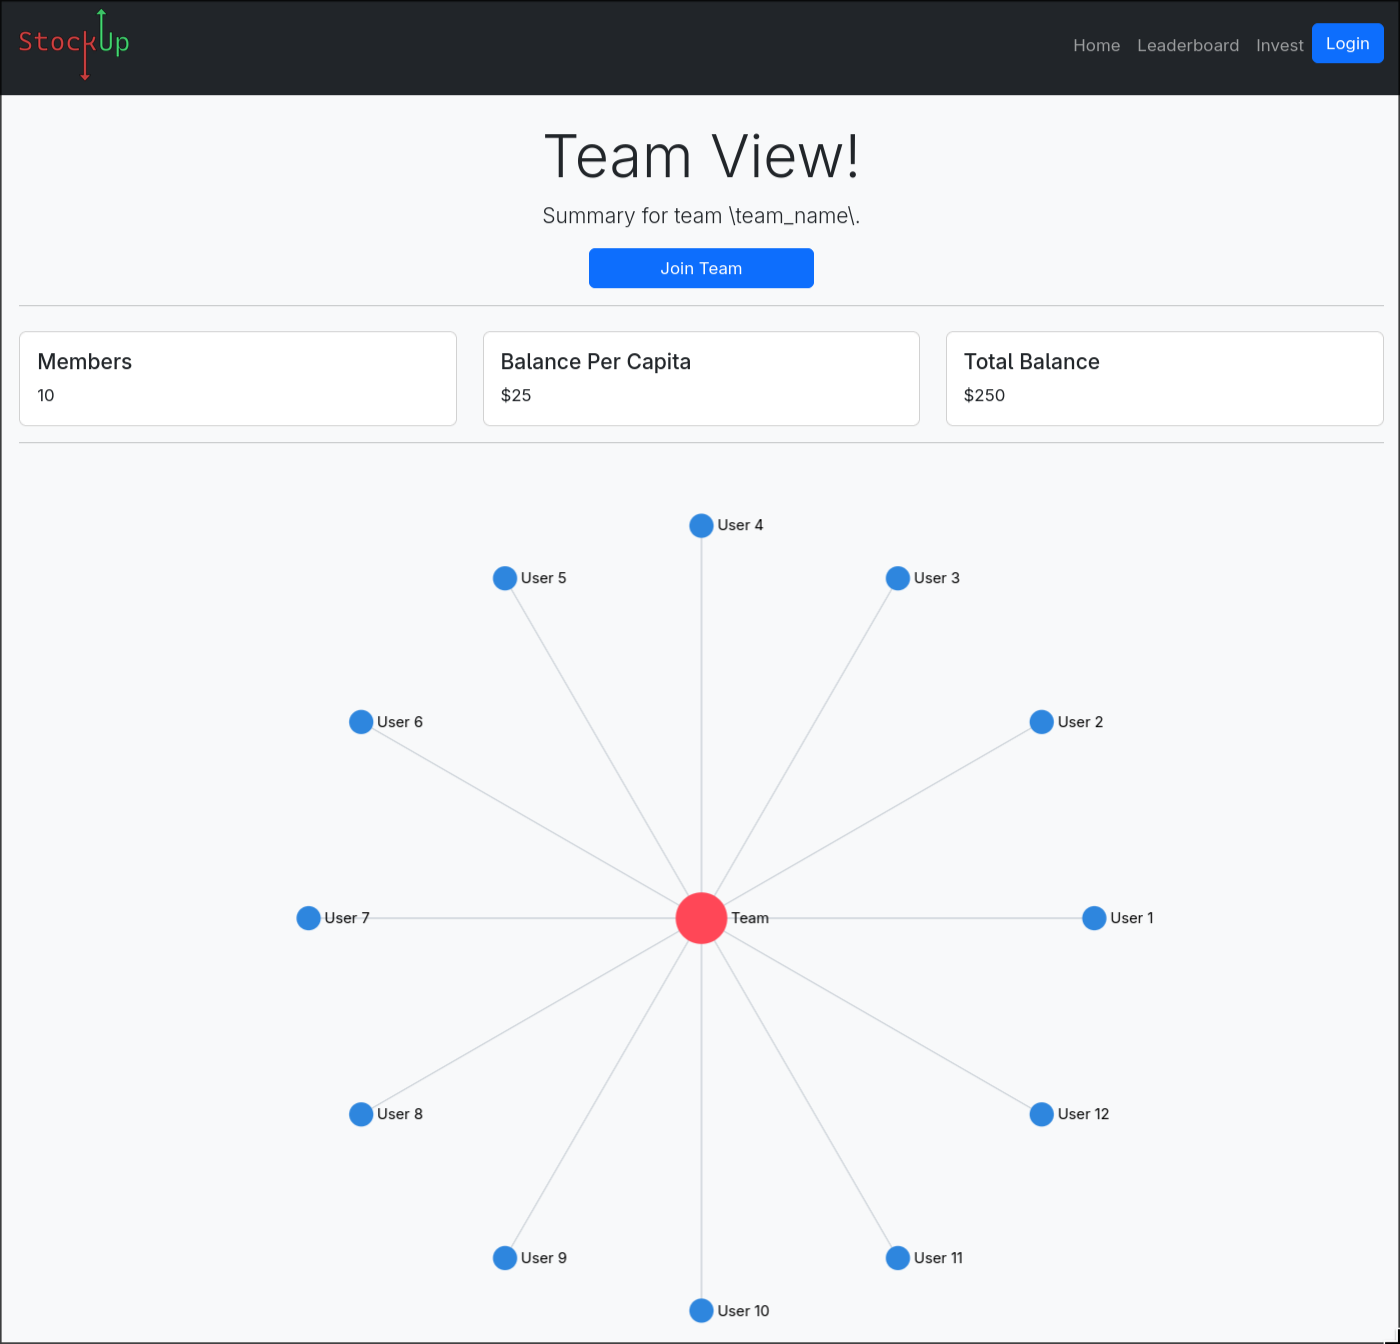
\includegraphics[width=0.7\linewidth]{image6.png}
        \caption{Co-Author Network}
        \label{fig:image6}
    \end{figure}

    \subsection{H-Index Filter}
    Our equivalent to the H-Index Filter is on the leaderboard page, where users can view the top performing teams and stocks.
    The H-Index Filter is defined to be "teams with a balance per capita greater than the mean balance per capita of all teams".
    These teams are shown in a graph.
    \begin{figure}[H]
        \centering
        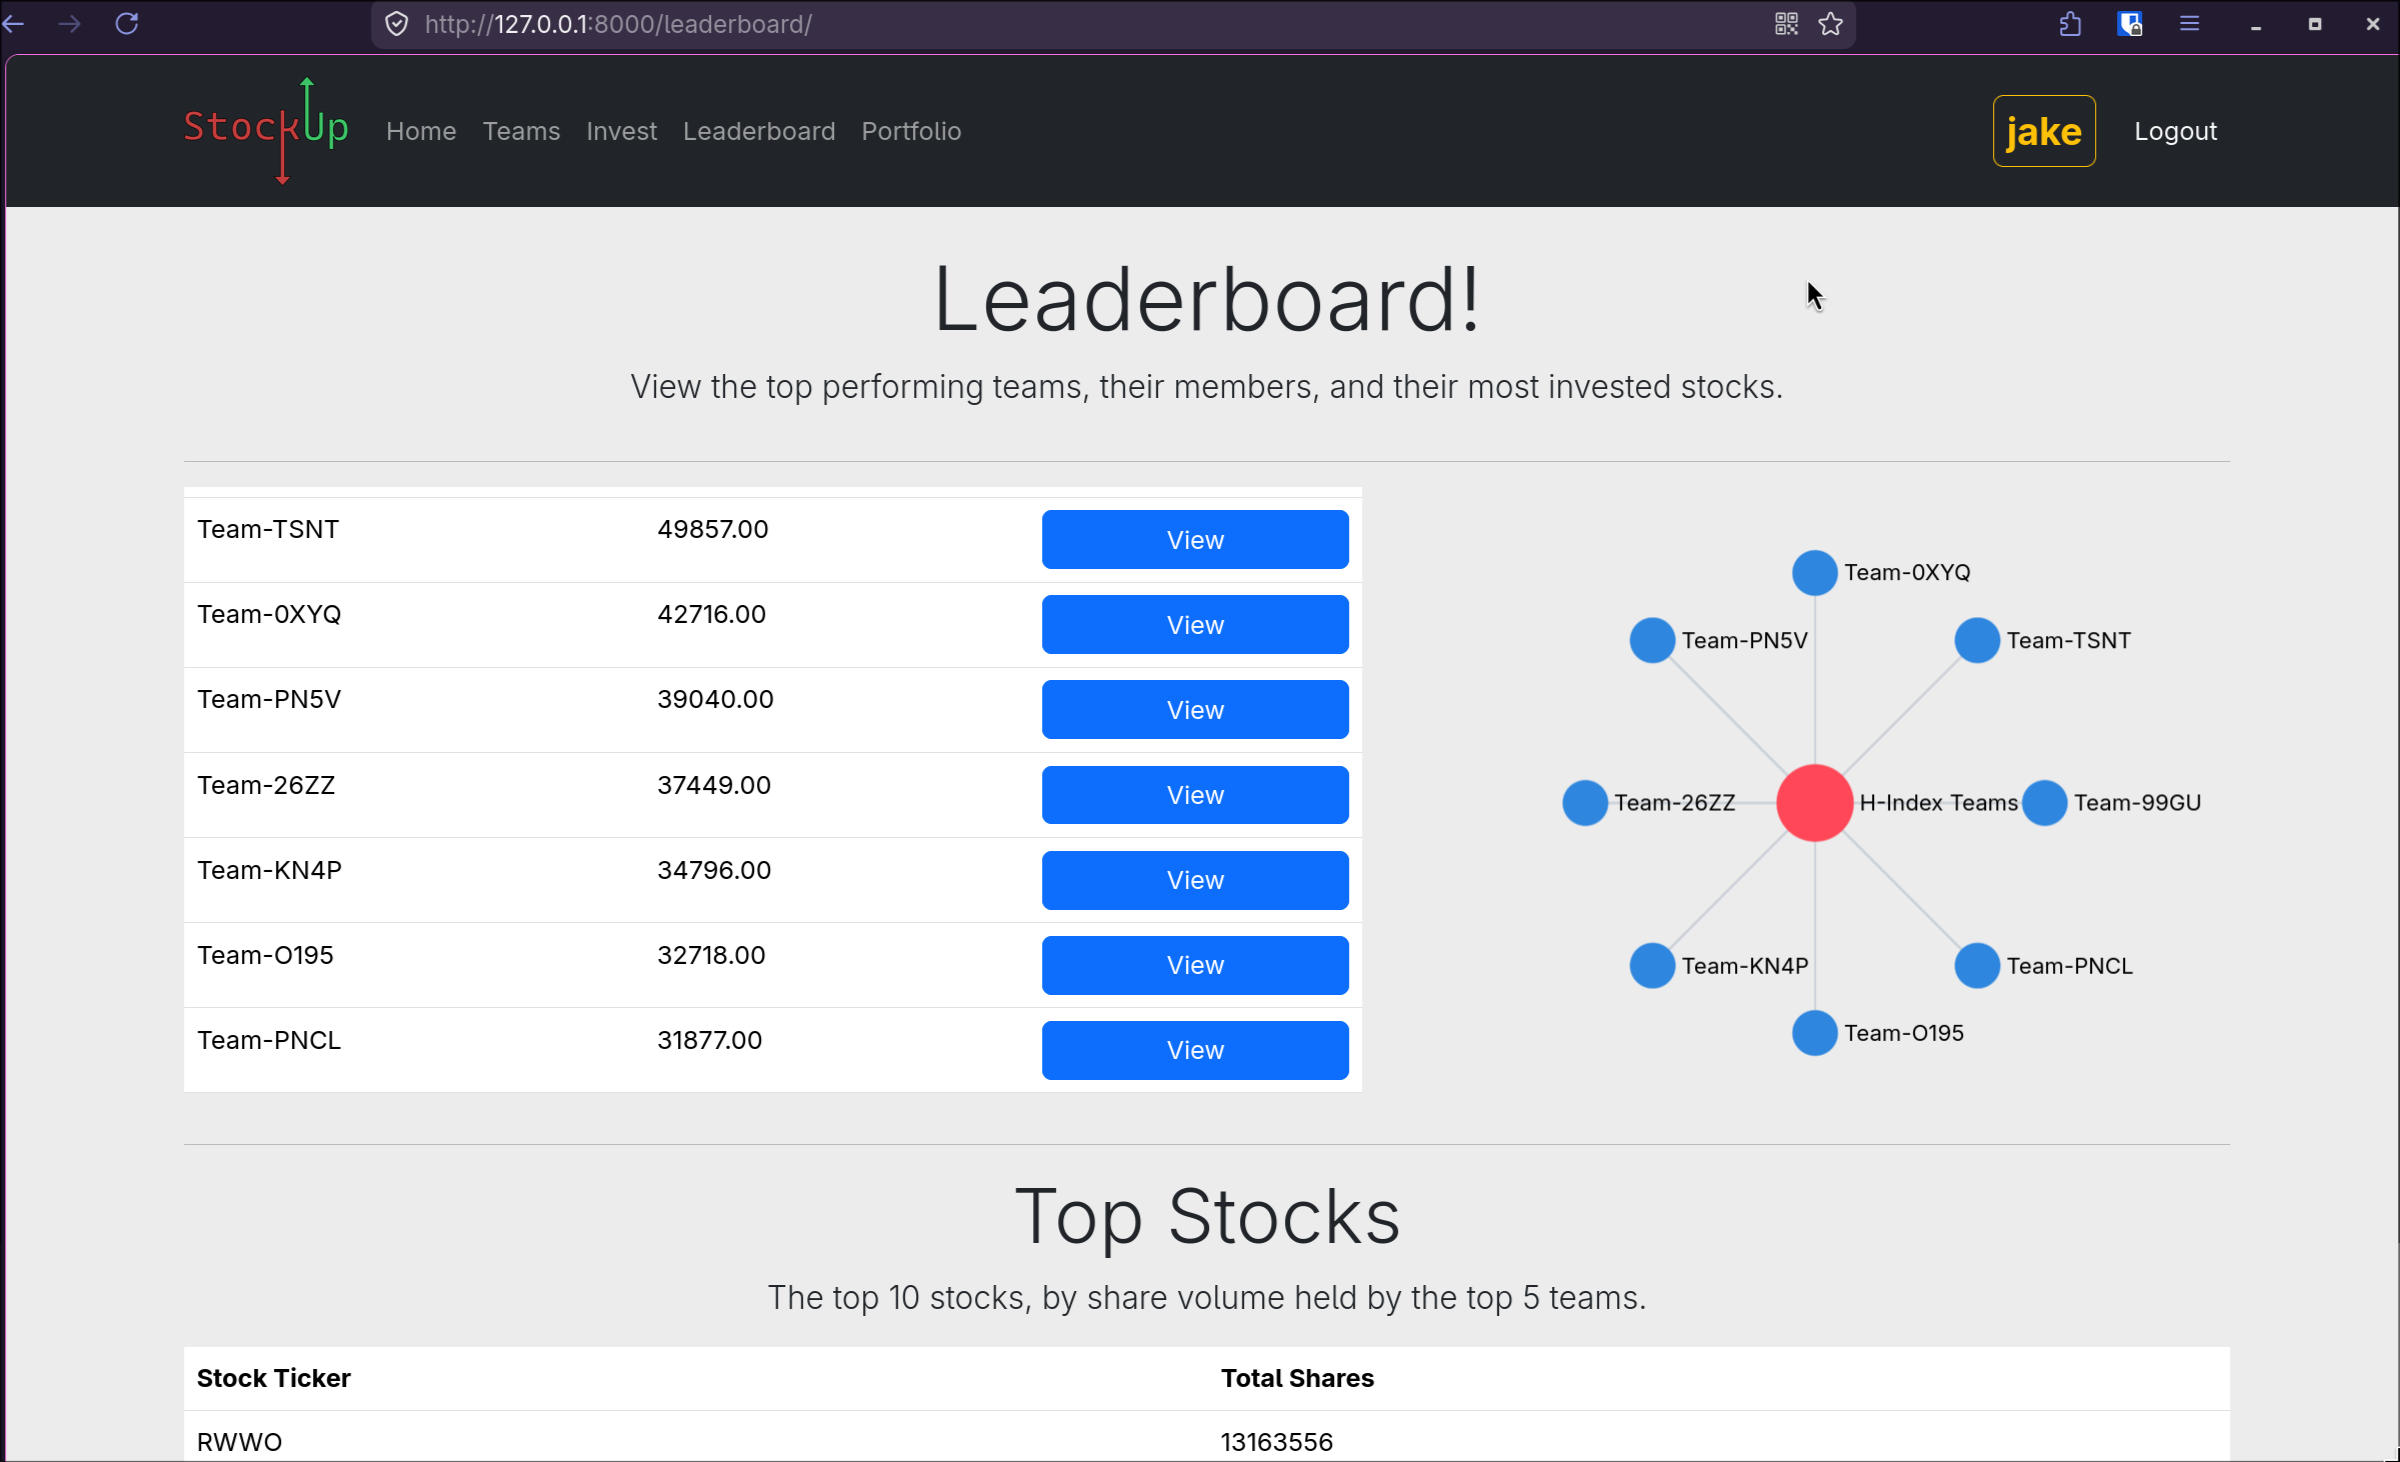
\includegraphics[width=0.7\linewidth]{leaderboard1.png}
        \caption{H-Index Filter}
        \label{fig:leaderboard1}
    \end{figure}

    \subsection{Q1 Journal Influence Network}
    Our equivalent to the Q1 Journal Influence Network is built upon the H-Index Filter. 
    It gets the teams that are in the H-Index, gets the users of those teams, then gets the top 10 stocks, by volume, held by the users of the team.
    The user can zoom in any team node in the H-Index Filter Graph to view the Q1 Journal Influence Network Graph of that team.
    \begin{figure}[H]
        \centering
        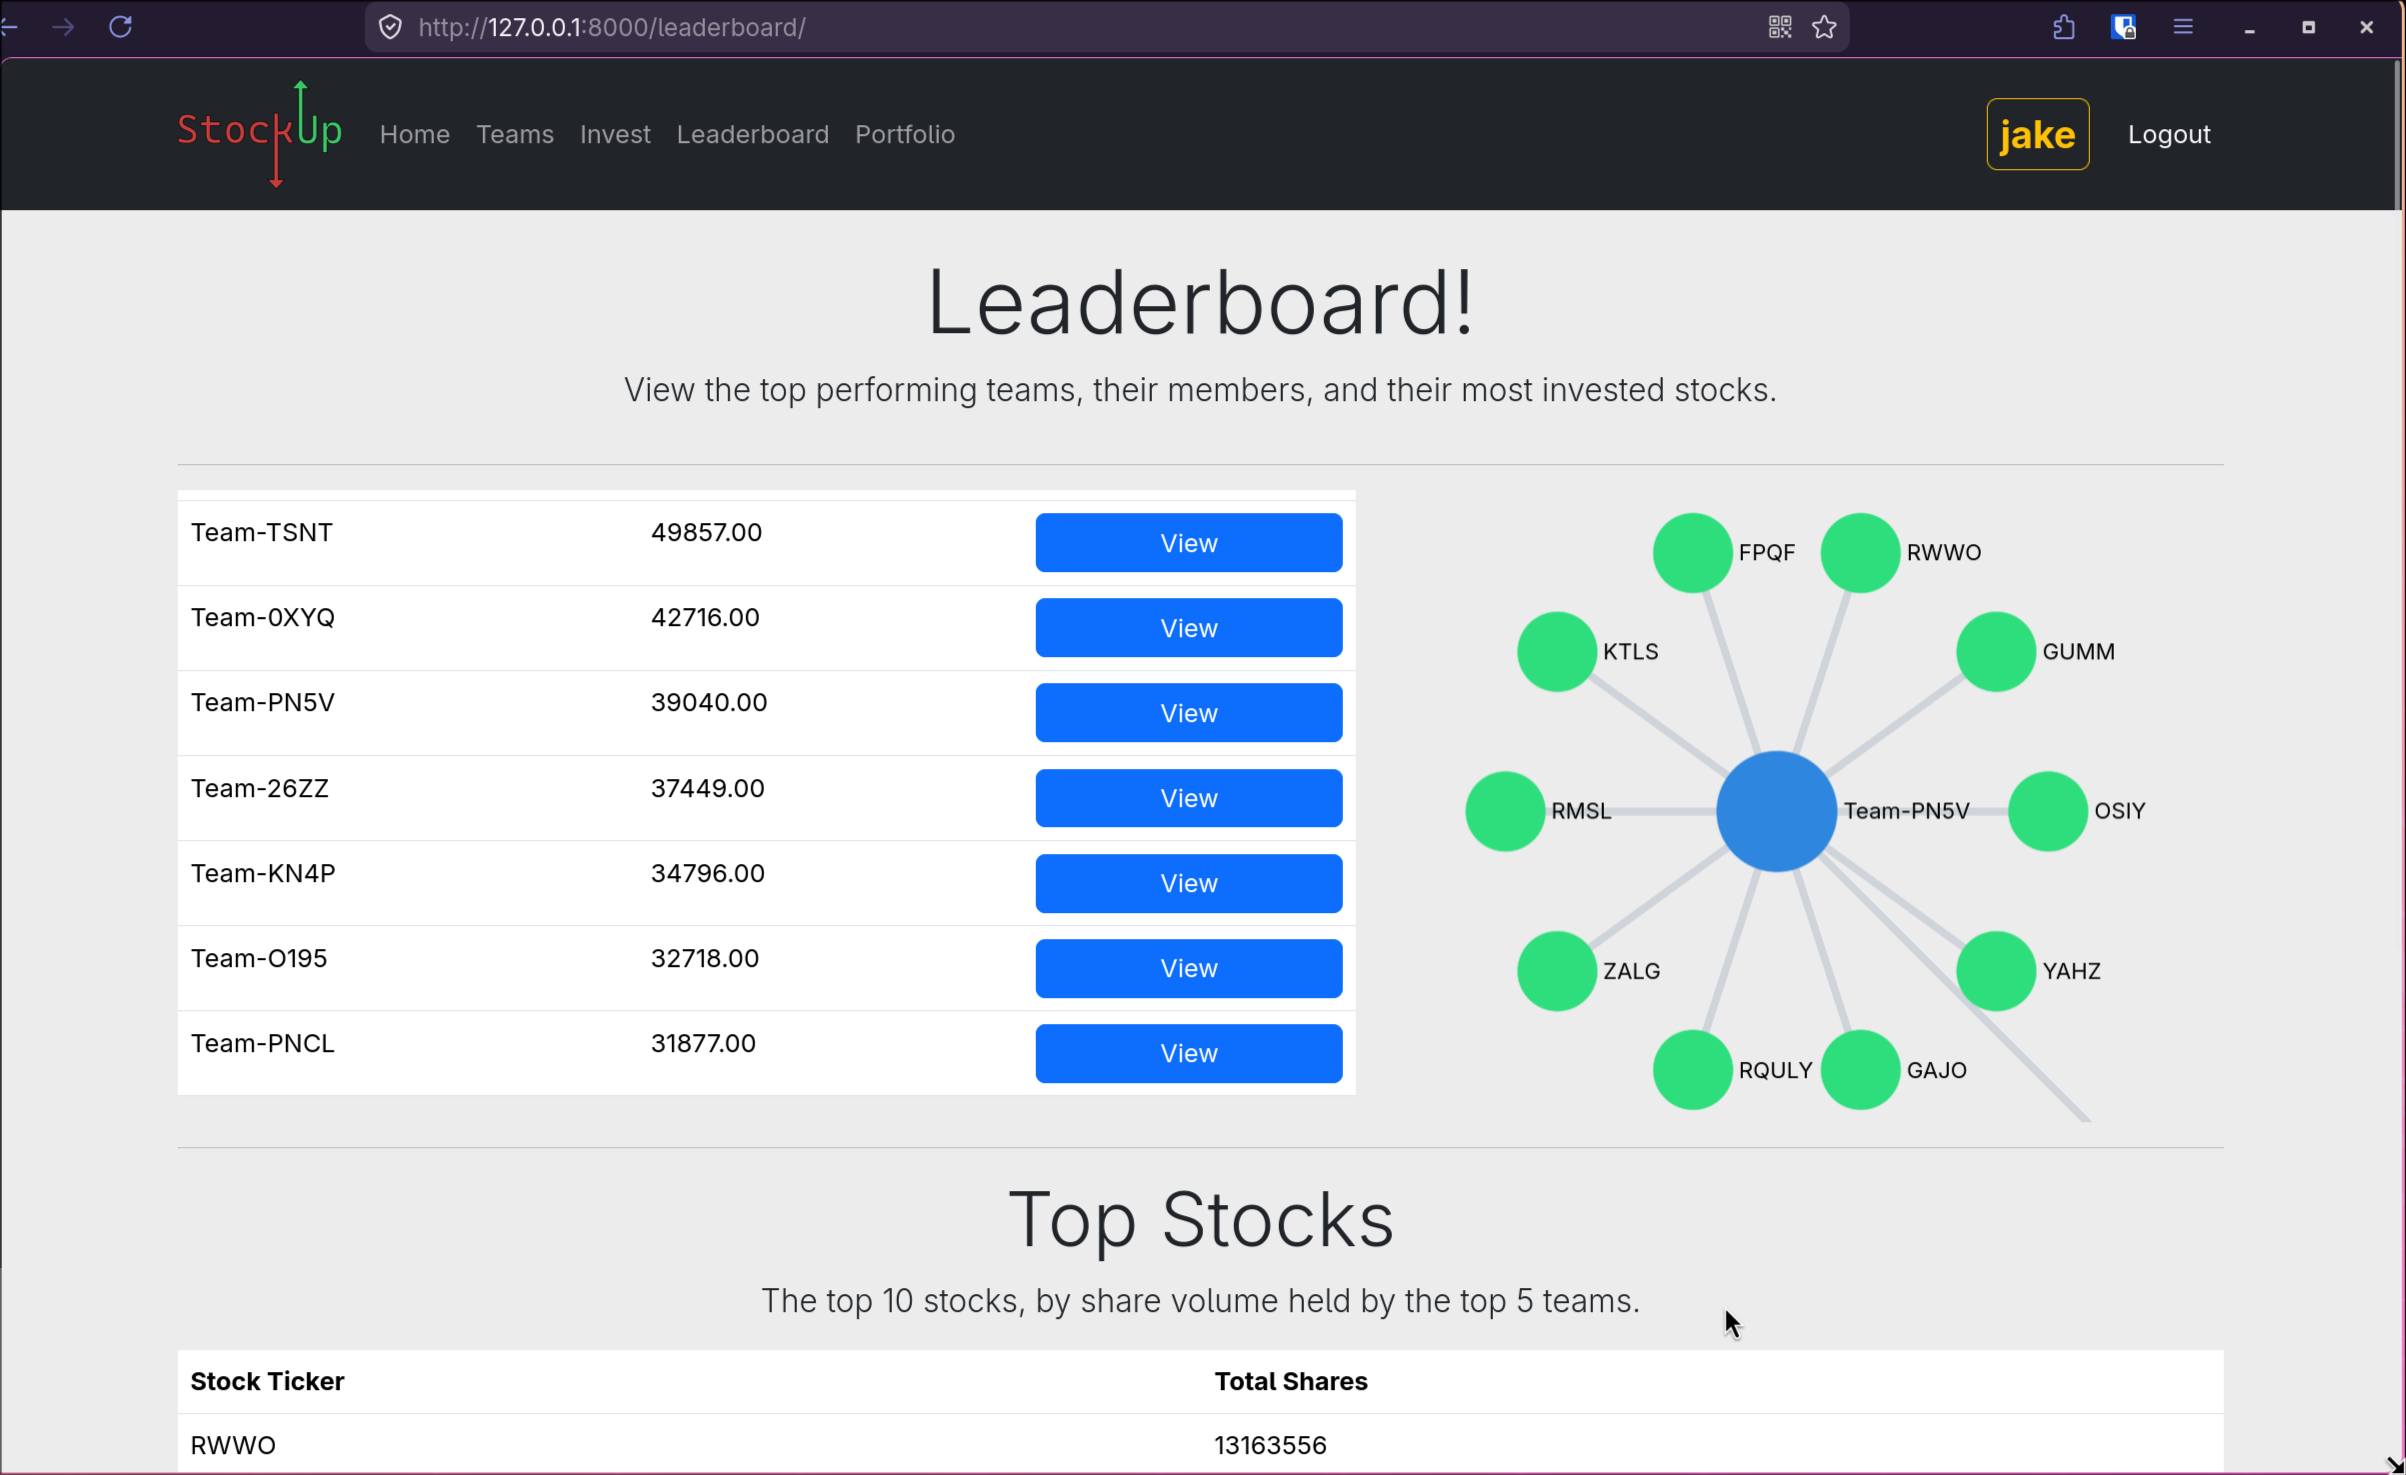
\includegraphics[width=0.7\linewidth]{leaderboard2.png}
        \caption{Q1 Journal Influence Network}
        \label{fig:leaderboard2}
    \end{figure}

\section{Deviations From the Original Plan}
    While our project execution has remained largely as planned, there have been a few small things that have changed.
    \begin{itemize}
        \item Initially, the plan was that the leaderboard and team page would be the same. That turned out to be too much info for a single page.
        \item An attribute has been added to the team entity, which is an owner field. This allows the owner to delete the team if they made it.
    \end{itemize}

\section{Progress Reports}
    \subsection{Phase I}
        \begin{itemize}
            \item Frontend design done - currently hardcoded in for the presentation.
            \item Database implemented in Django ORM.
            \item Basic backend implemented, does not interact with database.
        \end{itemize}

    \subsection{Phase II}
        \begin{itemize}
            \item Backend and database integrated with frontend.
            \item Implemented Co-Author Network graph.
            \item Implemented portfolio page.
        \end{itemize}

    \subsection{Phase III}
        \begin{itemize}
            \item Reworked Leaderboard page.
            \item Implemented H-Index Filter and graph.
            \item Implemented Q1 Journal Influence Network and graph.
            \item Added login system and requirements to view pages.
        \end{itemize}

\section{Validation}
    \begin{figure}[H]
        \centering
        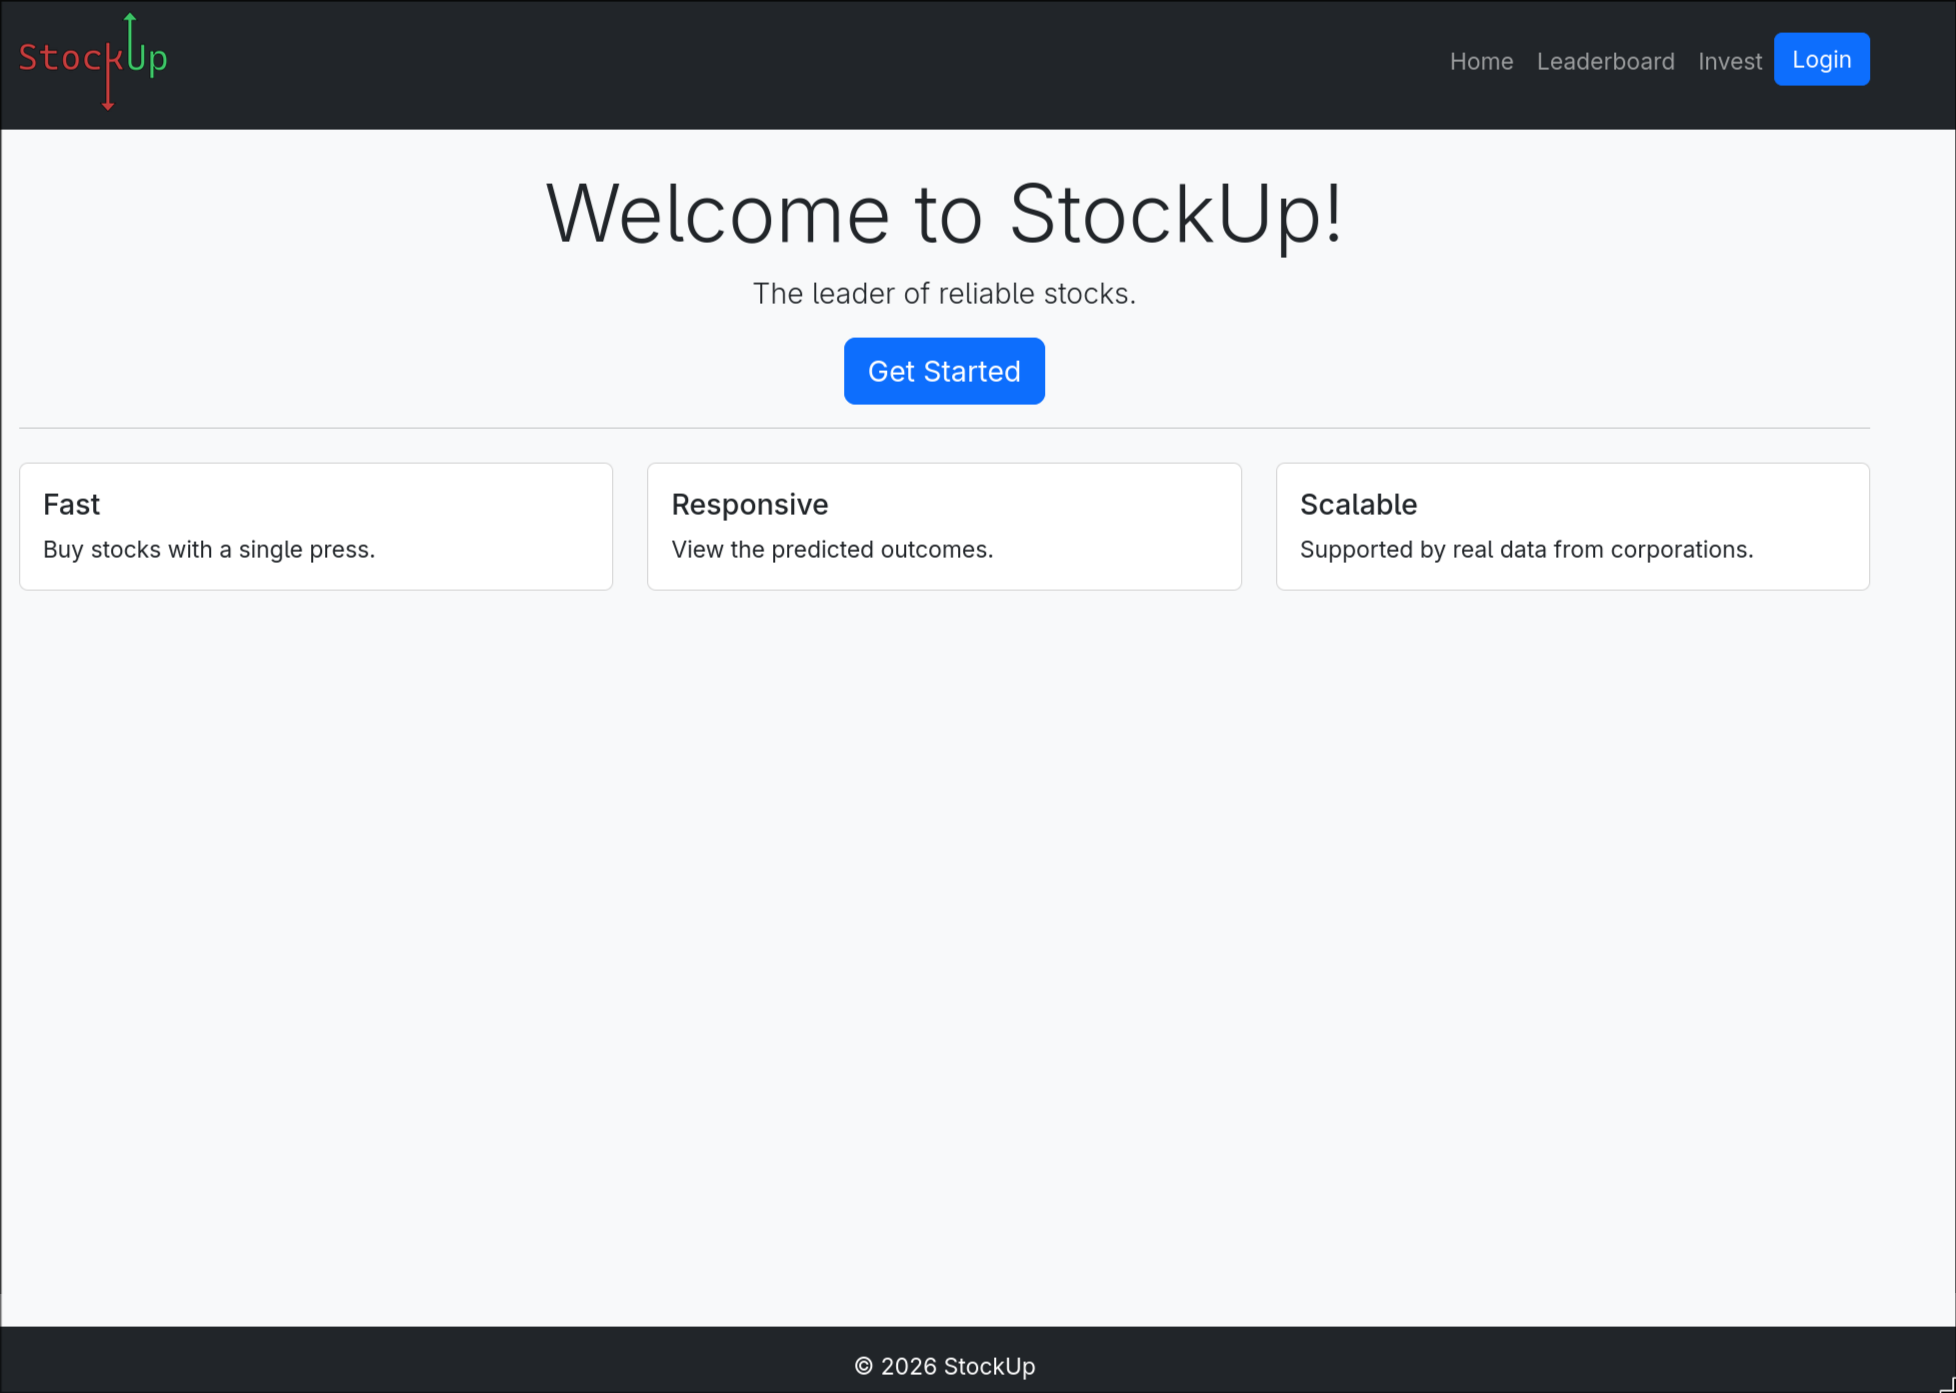
\includegraphics[width=0.7\linewidth]{image1.png}
        \caption{Home Page}
        \label{fig:image1}
    \end{figure}
    
    \begin{figure}[H]
        \centering
        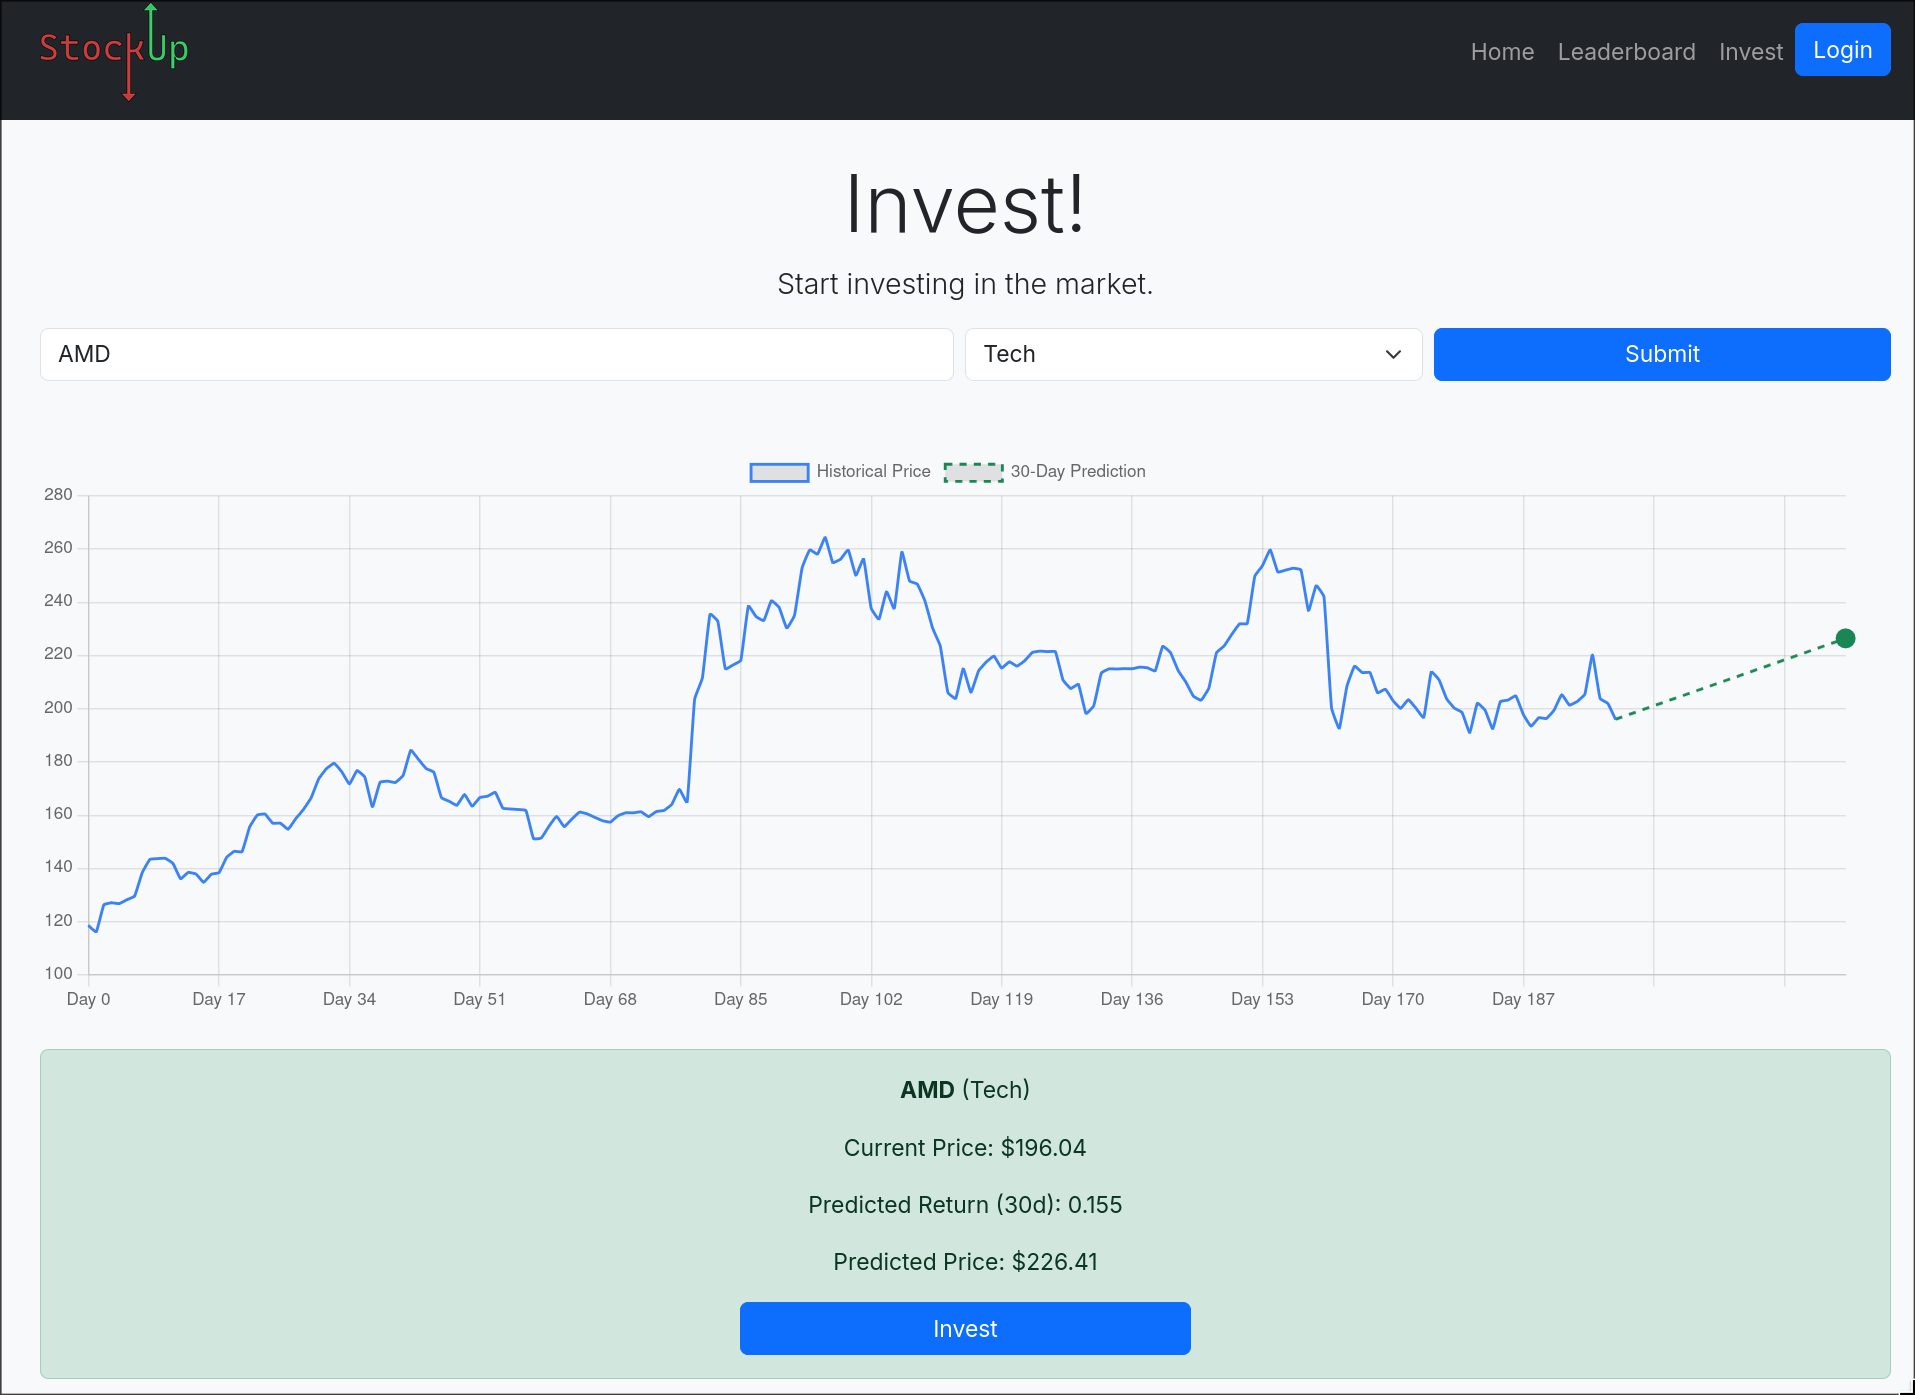
\includegraphics[width=0.7\linewidth]{image3.png}
        \caption{Stock Investing Page}
        \label{fig:image3}
    \end{figure}
    
    \begin{figure}[H]
        \centering
        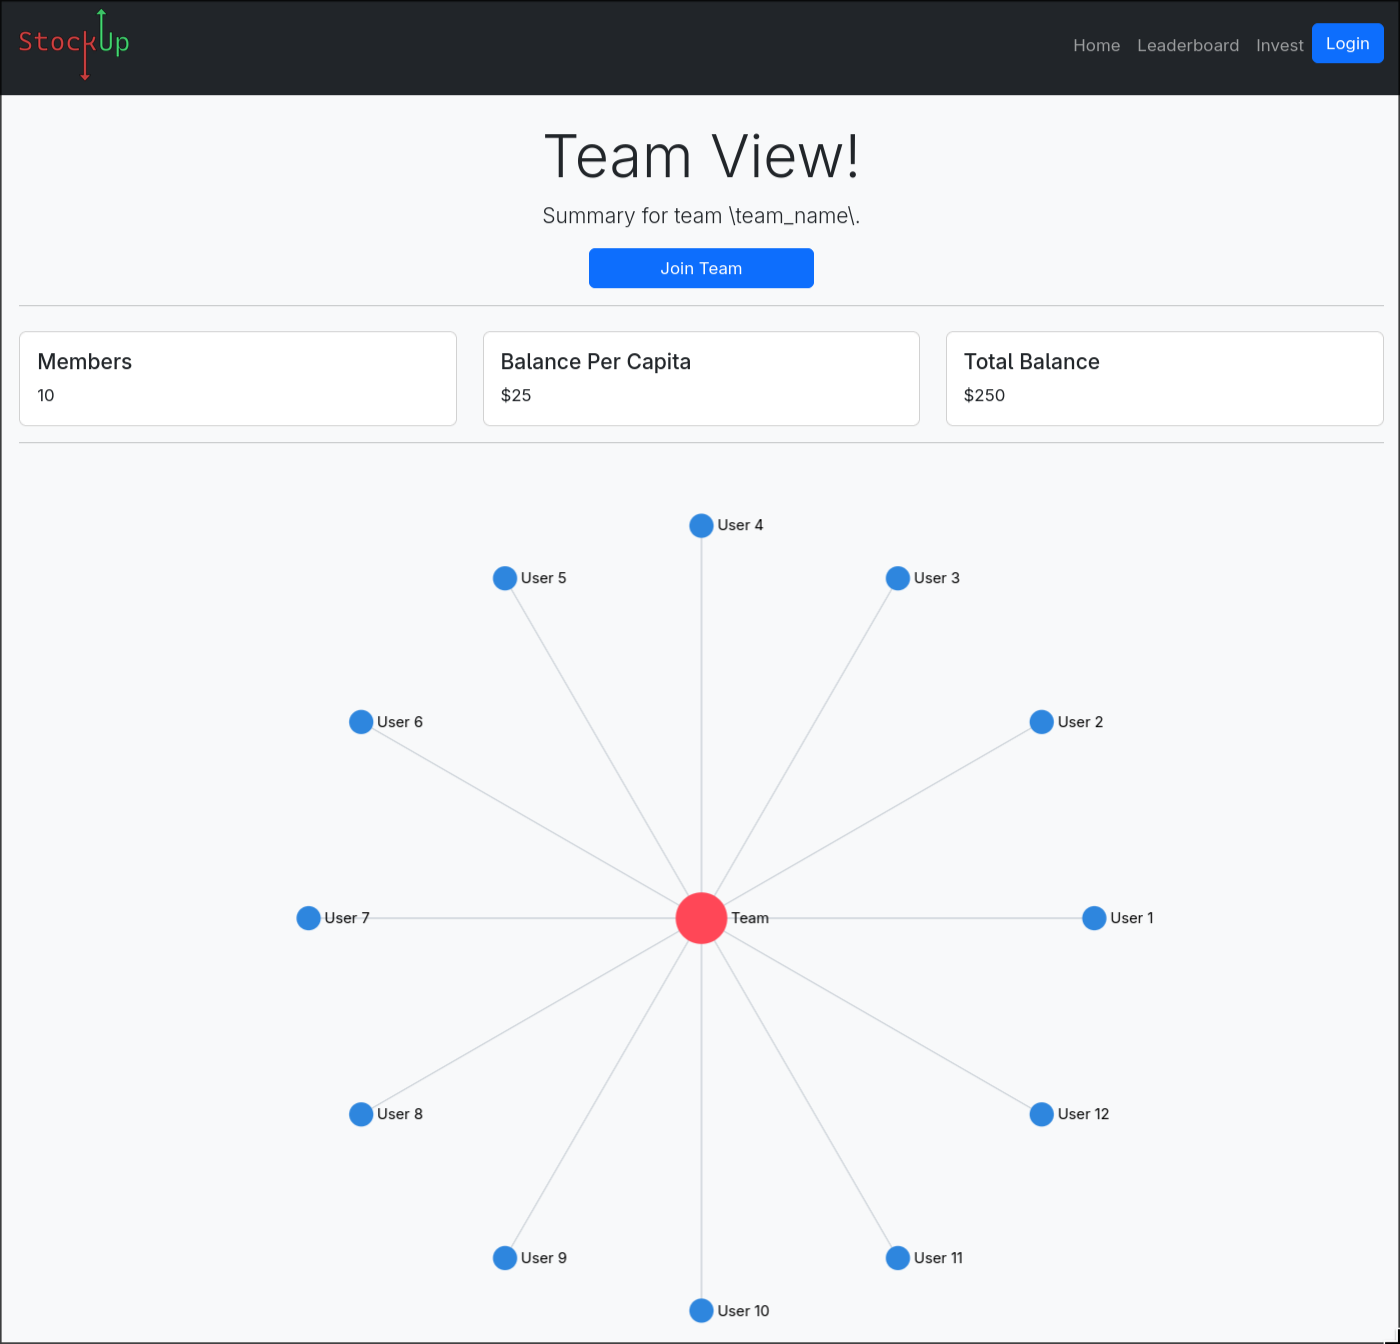
\includegraphics[width=0.7\linewidth]{image6.png}
        \caption{Team View Page}
        \label{fig:image6}
    \end{figure}
    
    \begin{figure}[H]
        \centering
        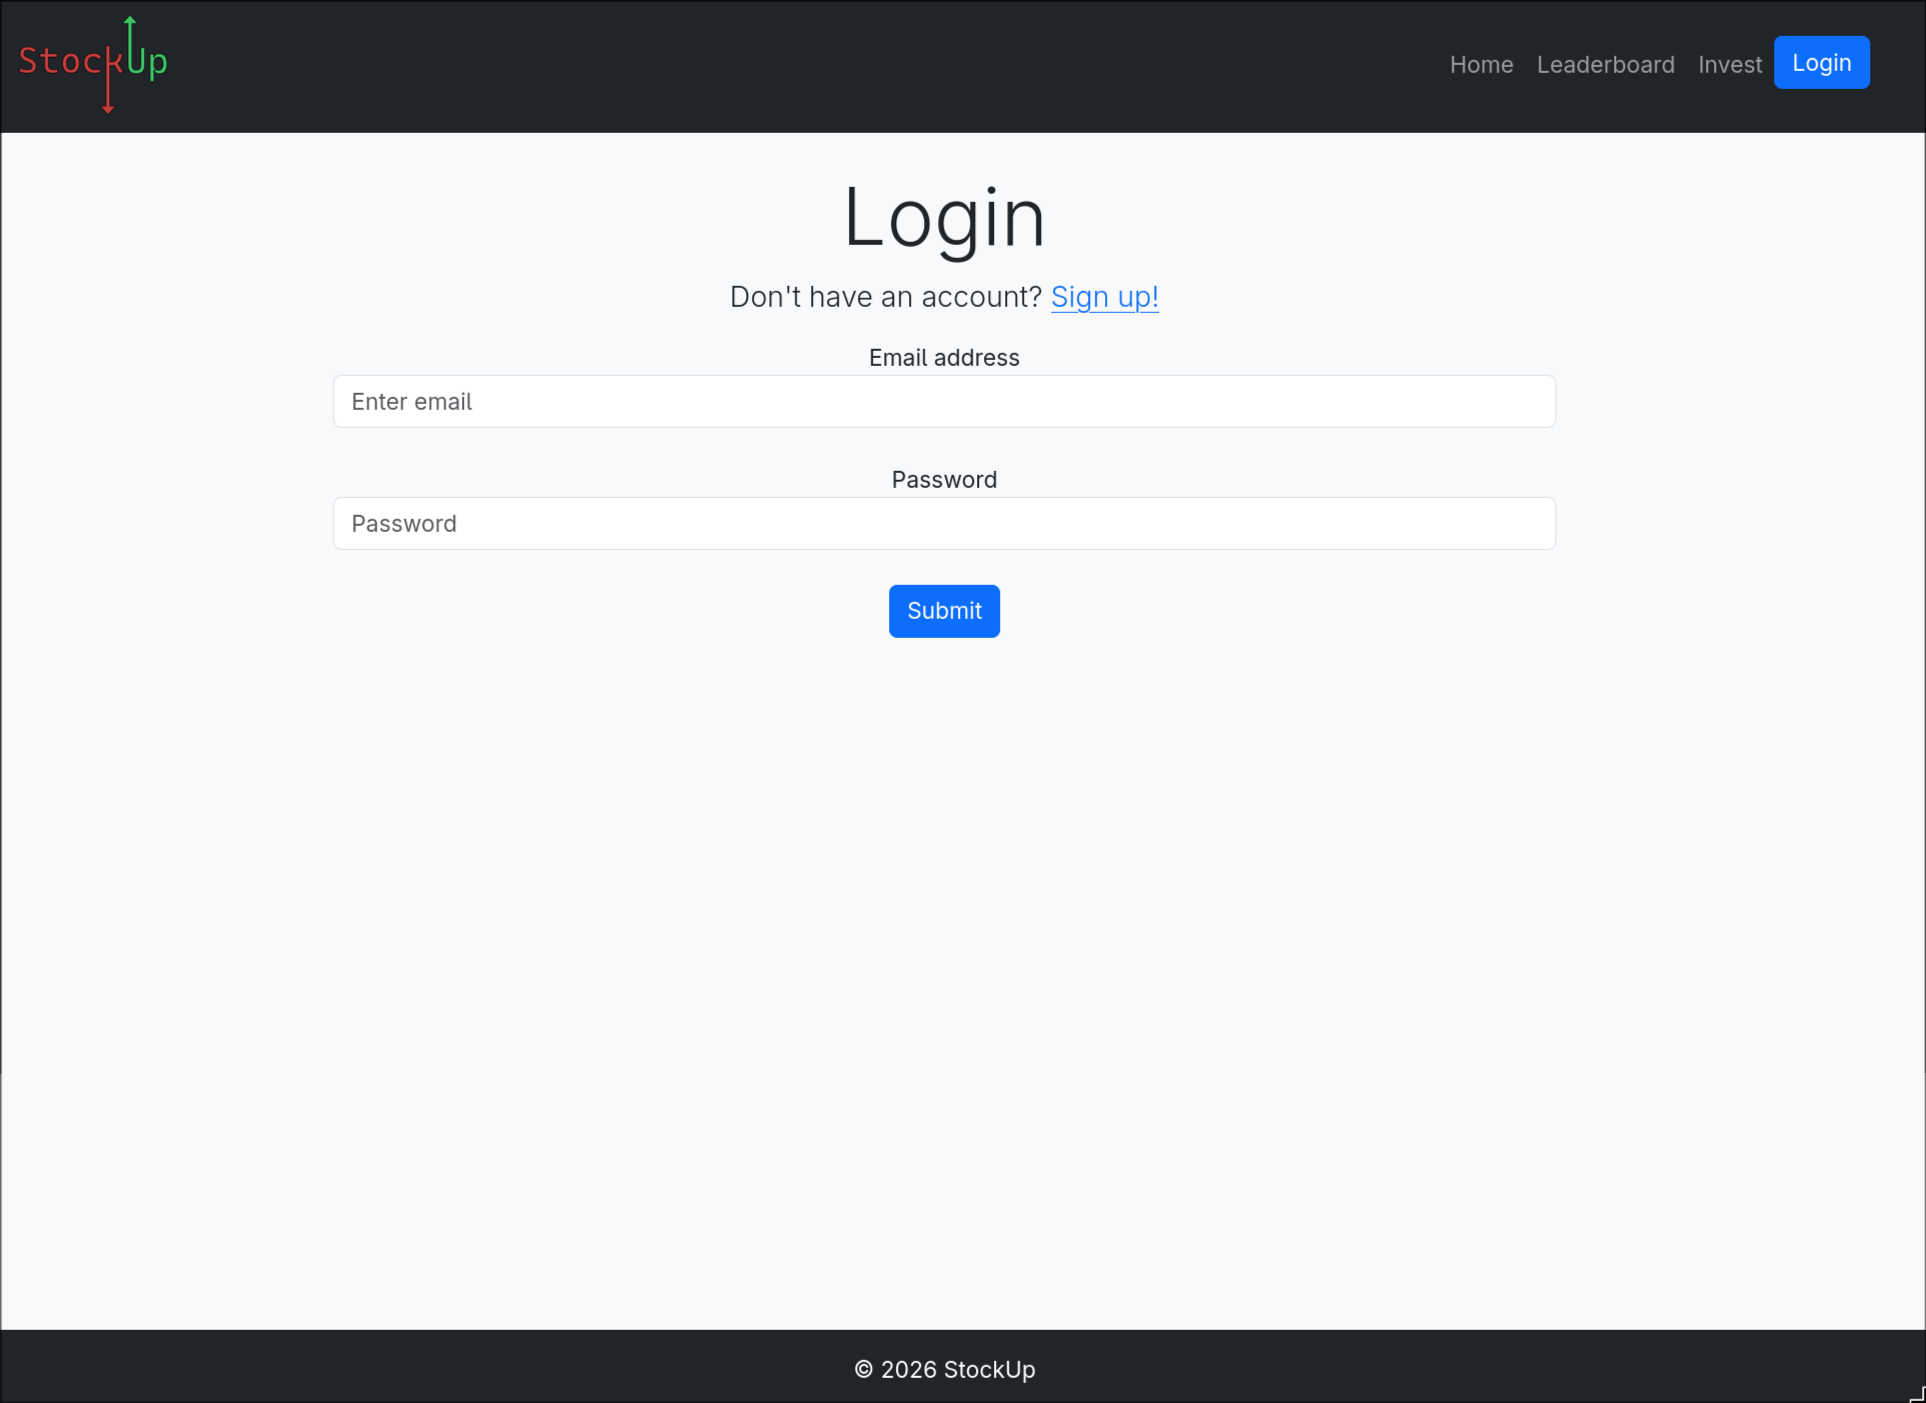
\includegraphics[width=0.7\linewidth]{image2.png}
        \caption{Login Page}
        \label{fig:image2}
    \end{figure}
    
    \begin{figure}[H]
        \centering
        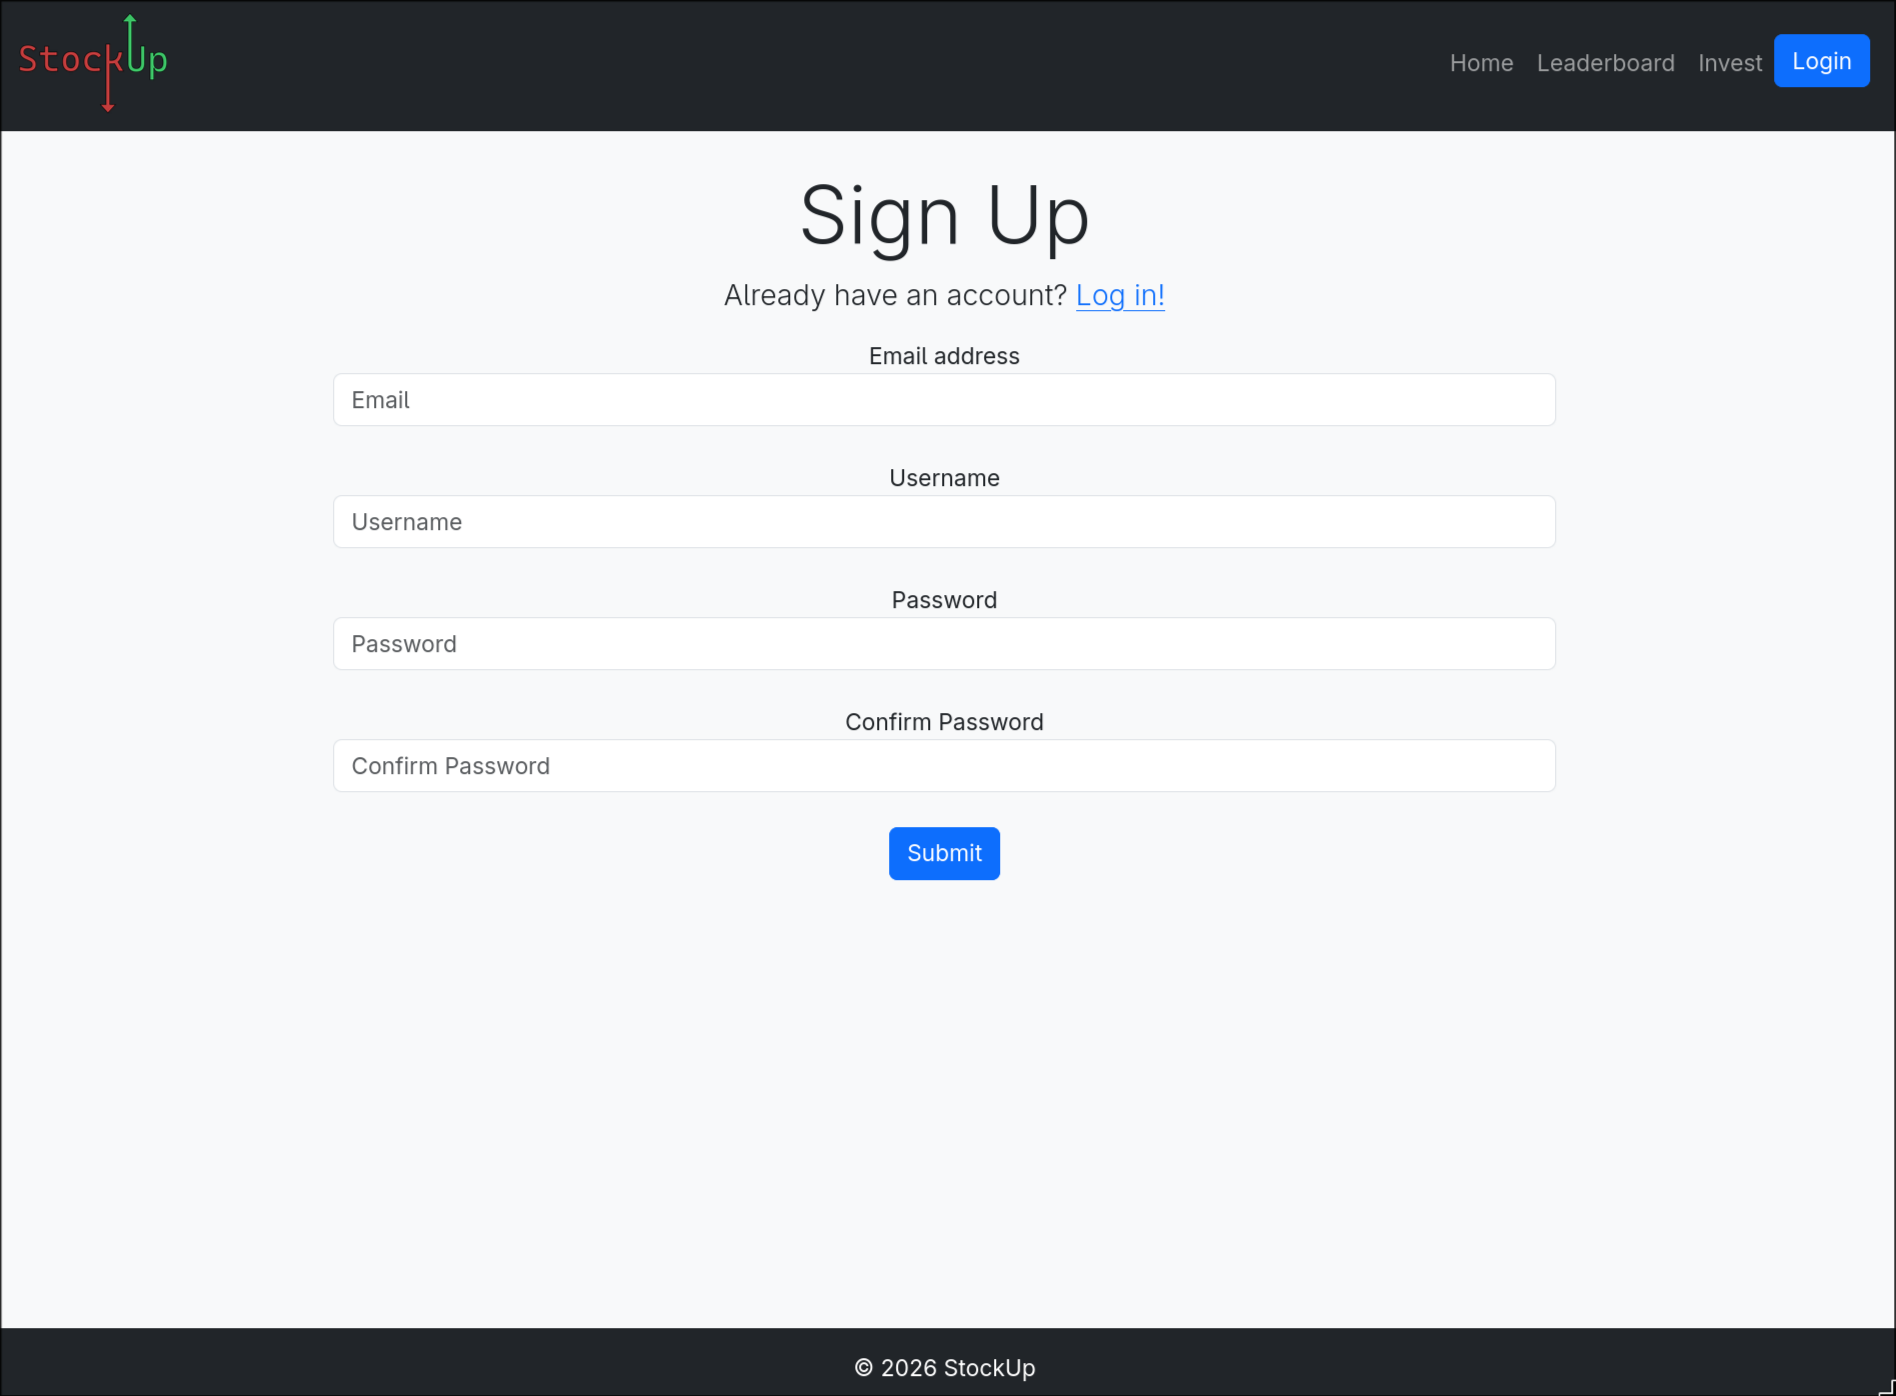
\includegraphics[width=0.7\linewidth]{image7.png}
        \caption{Sign Up Page}
        \label{fig:image7}
    \end{figure}
    
    \begin{figure}[H]
        \centering
        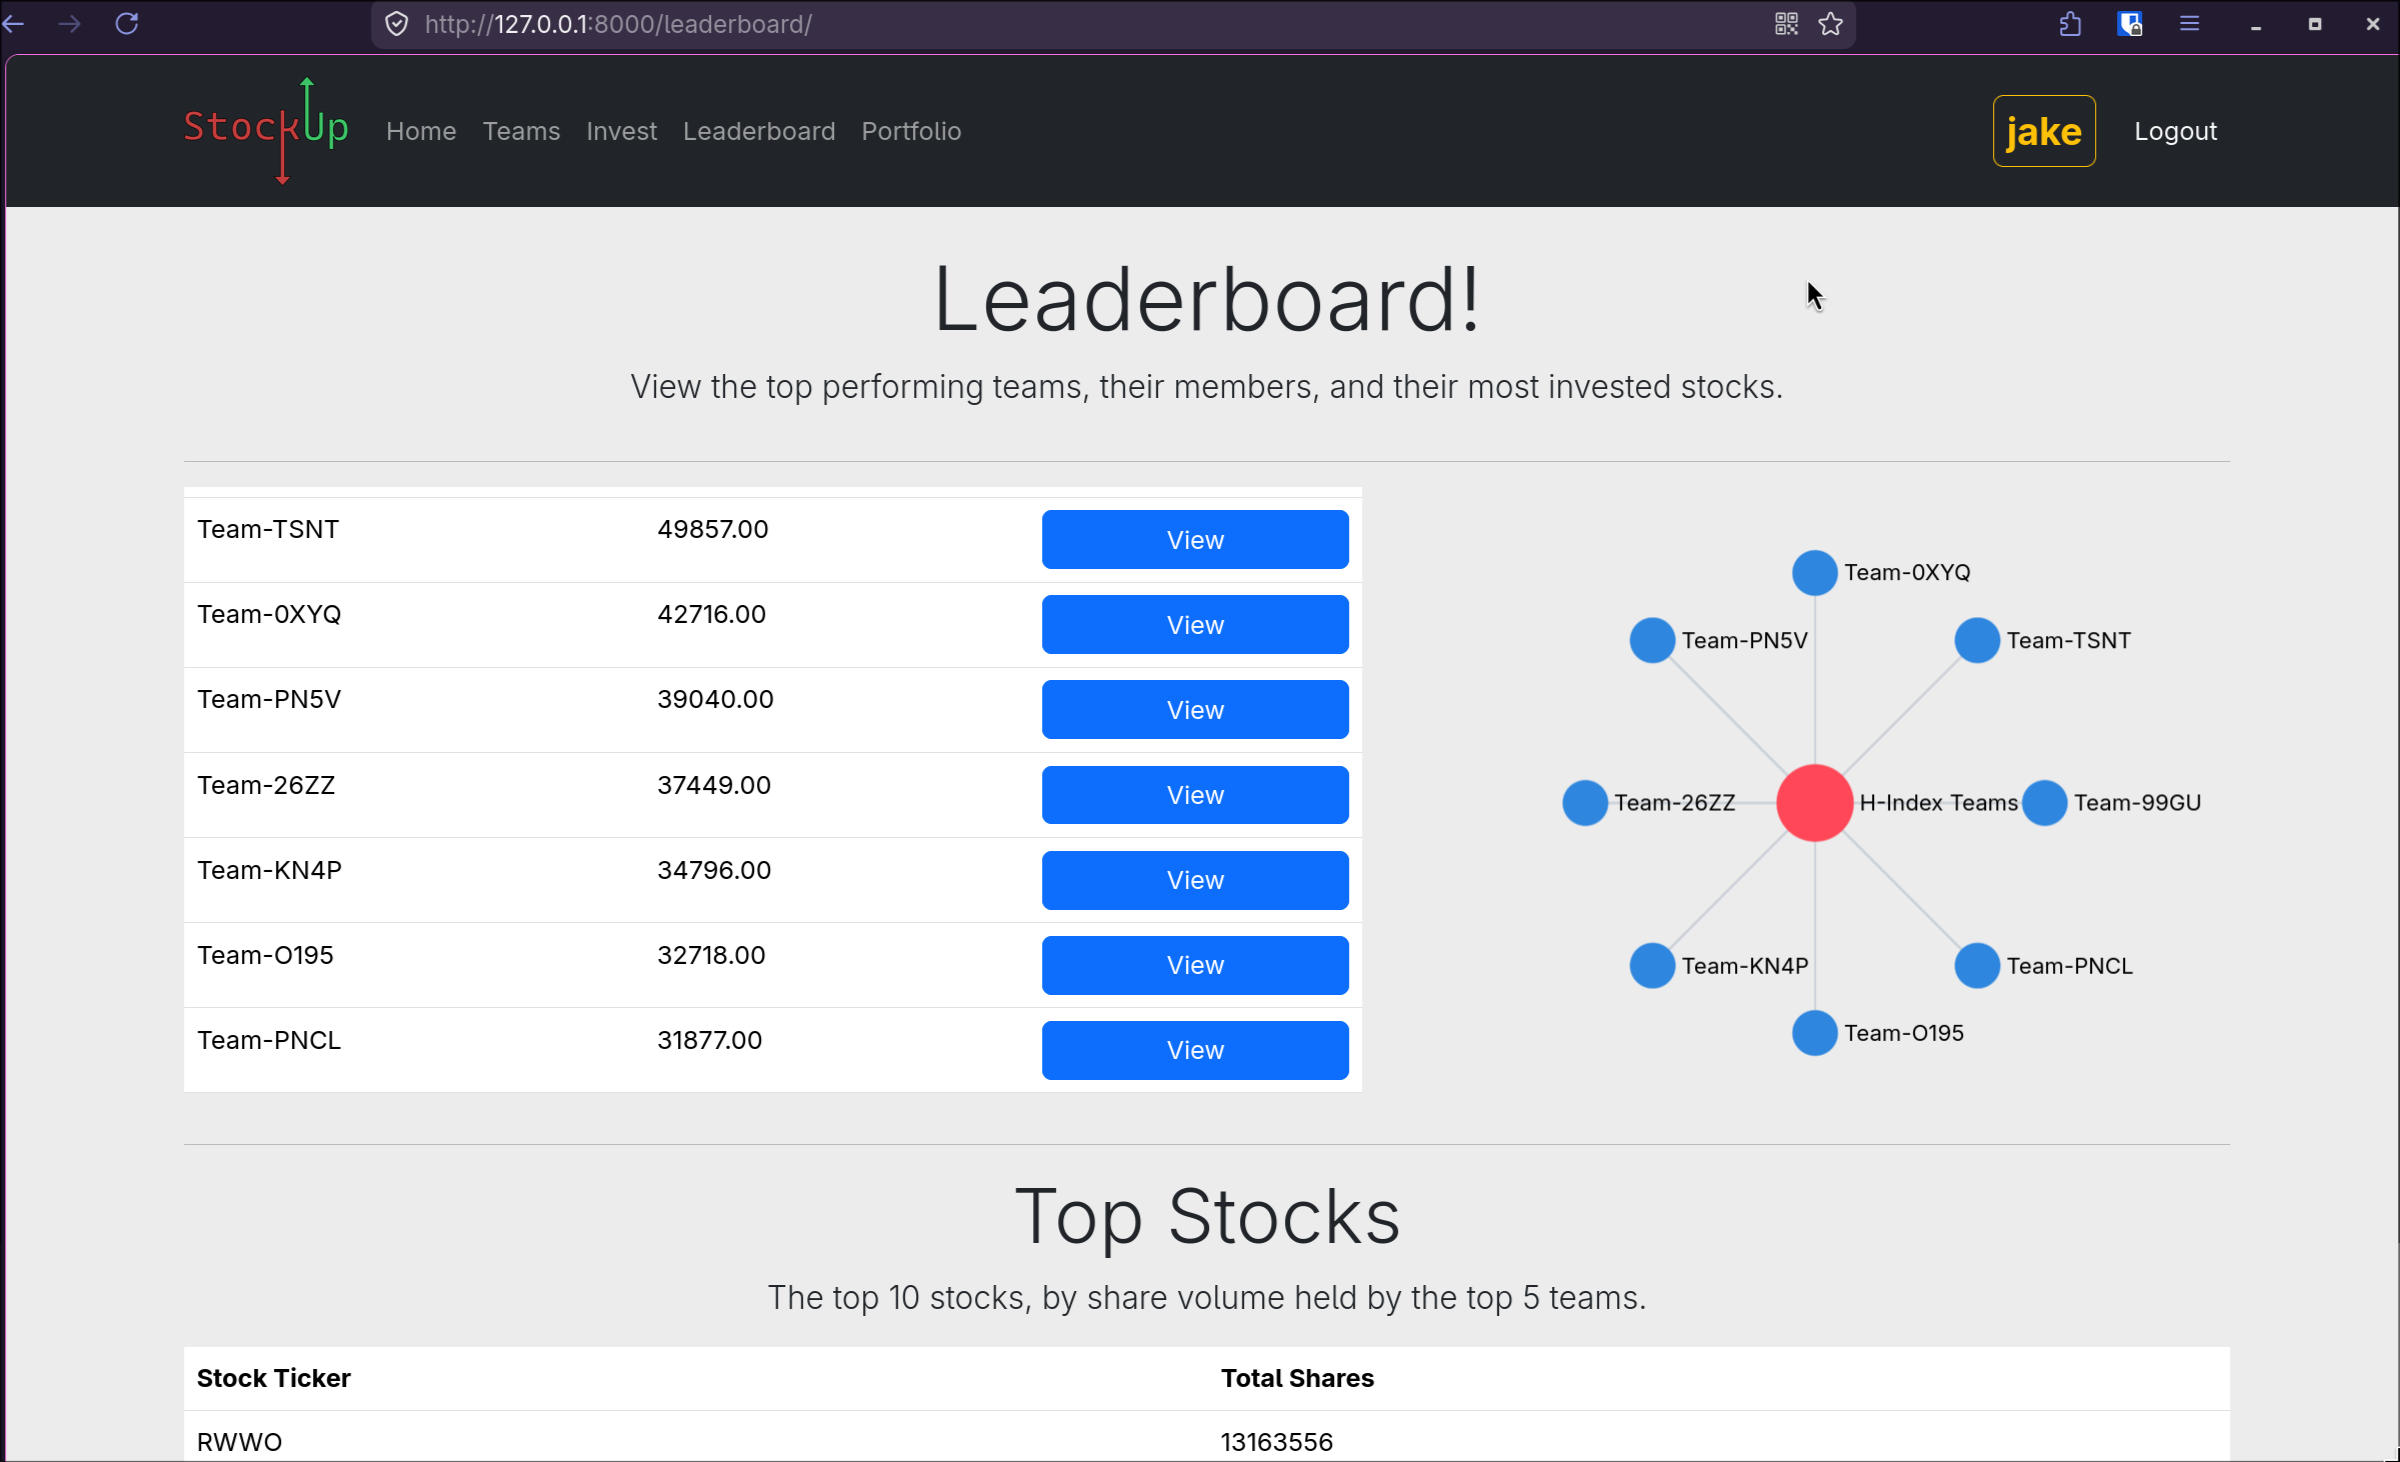
\includegraphics[width=0.7\linewidth]{leaderboard1.png}
        \caption{Leaderboards Page}
        \label{fig:image8}
    \end{figure}
    
    \begin{figure}[H]
        \centering
        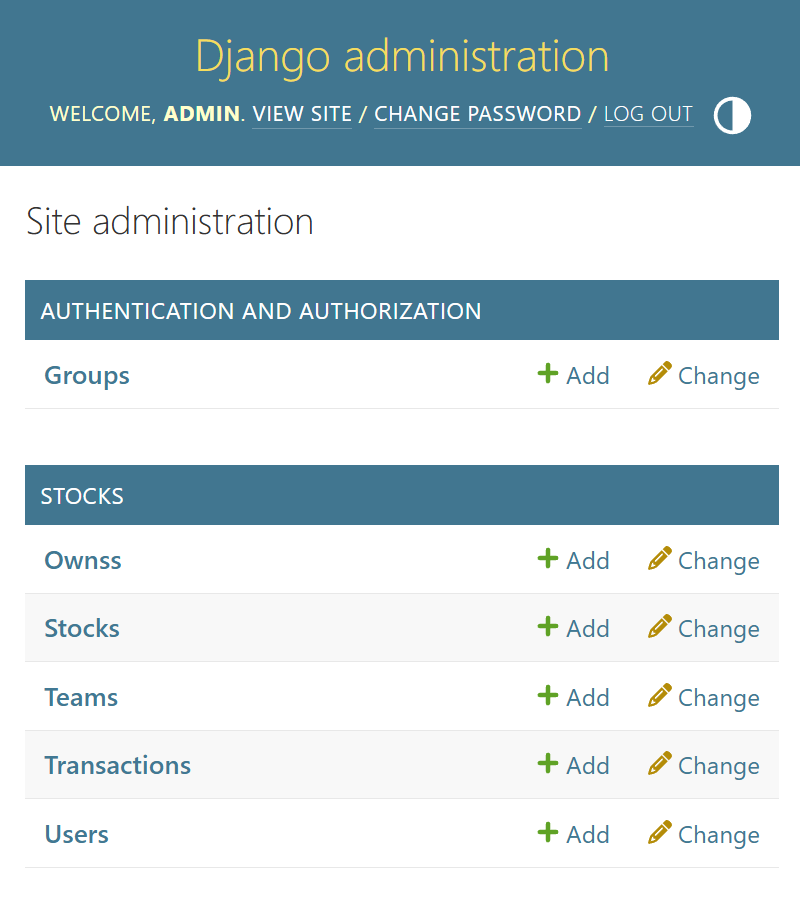
\includegraphics[width=0.6\linewidth]{image5.png}
        \caption{Database Administration Page}
        \label{fig:image5}
    \end{figure}

    \begin{figure}[H]
        \centering
        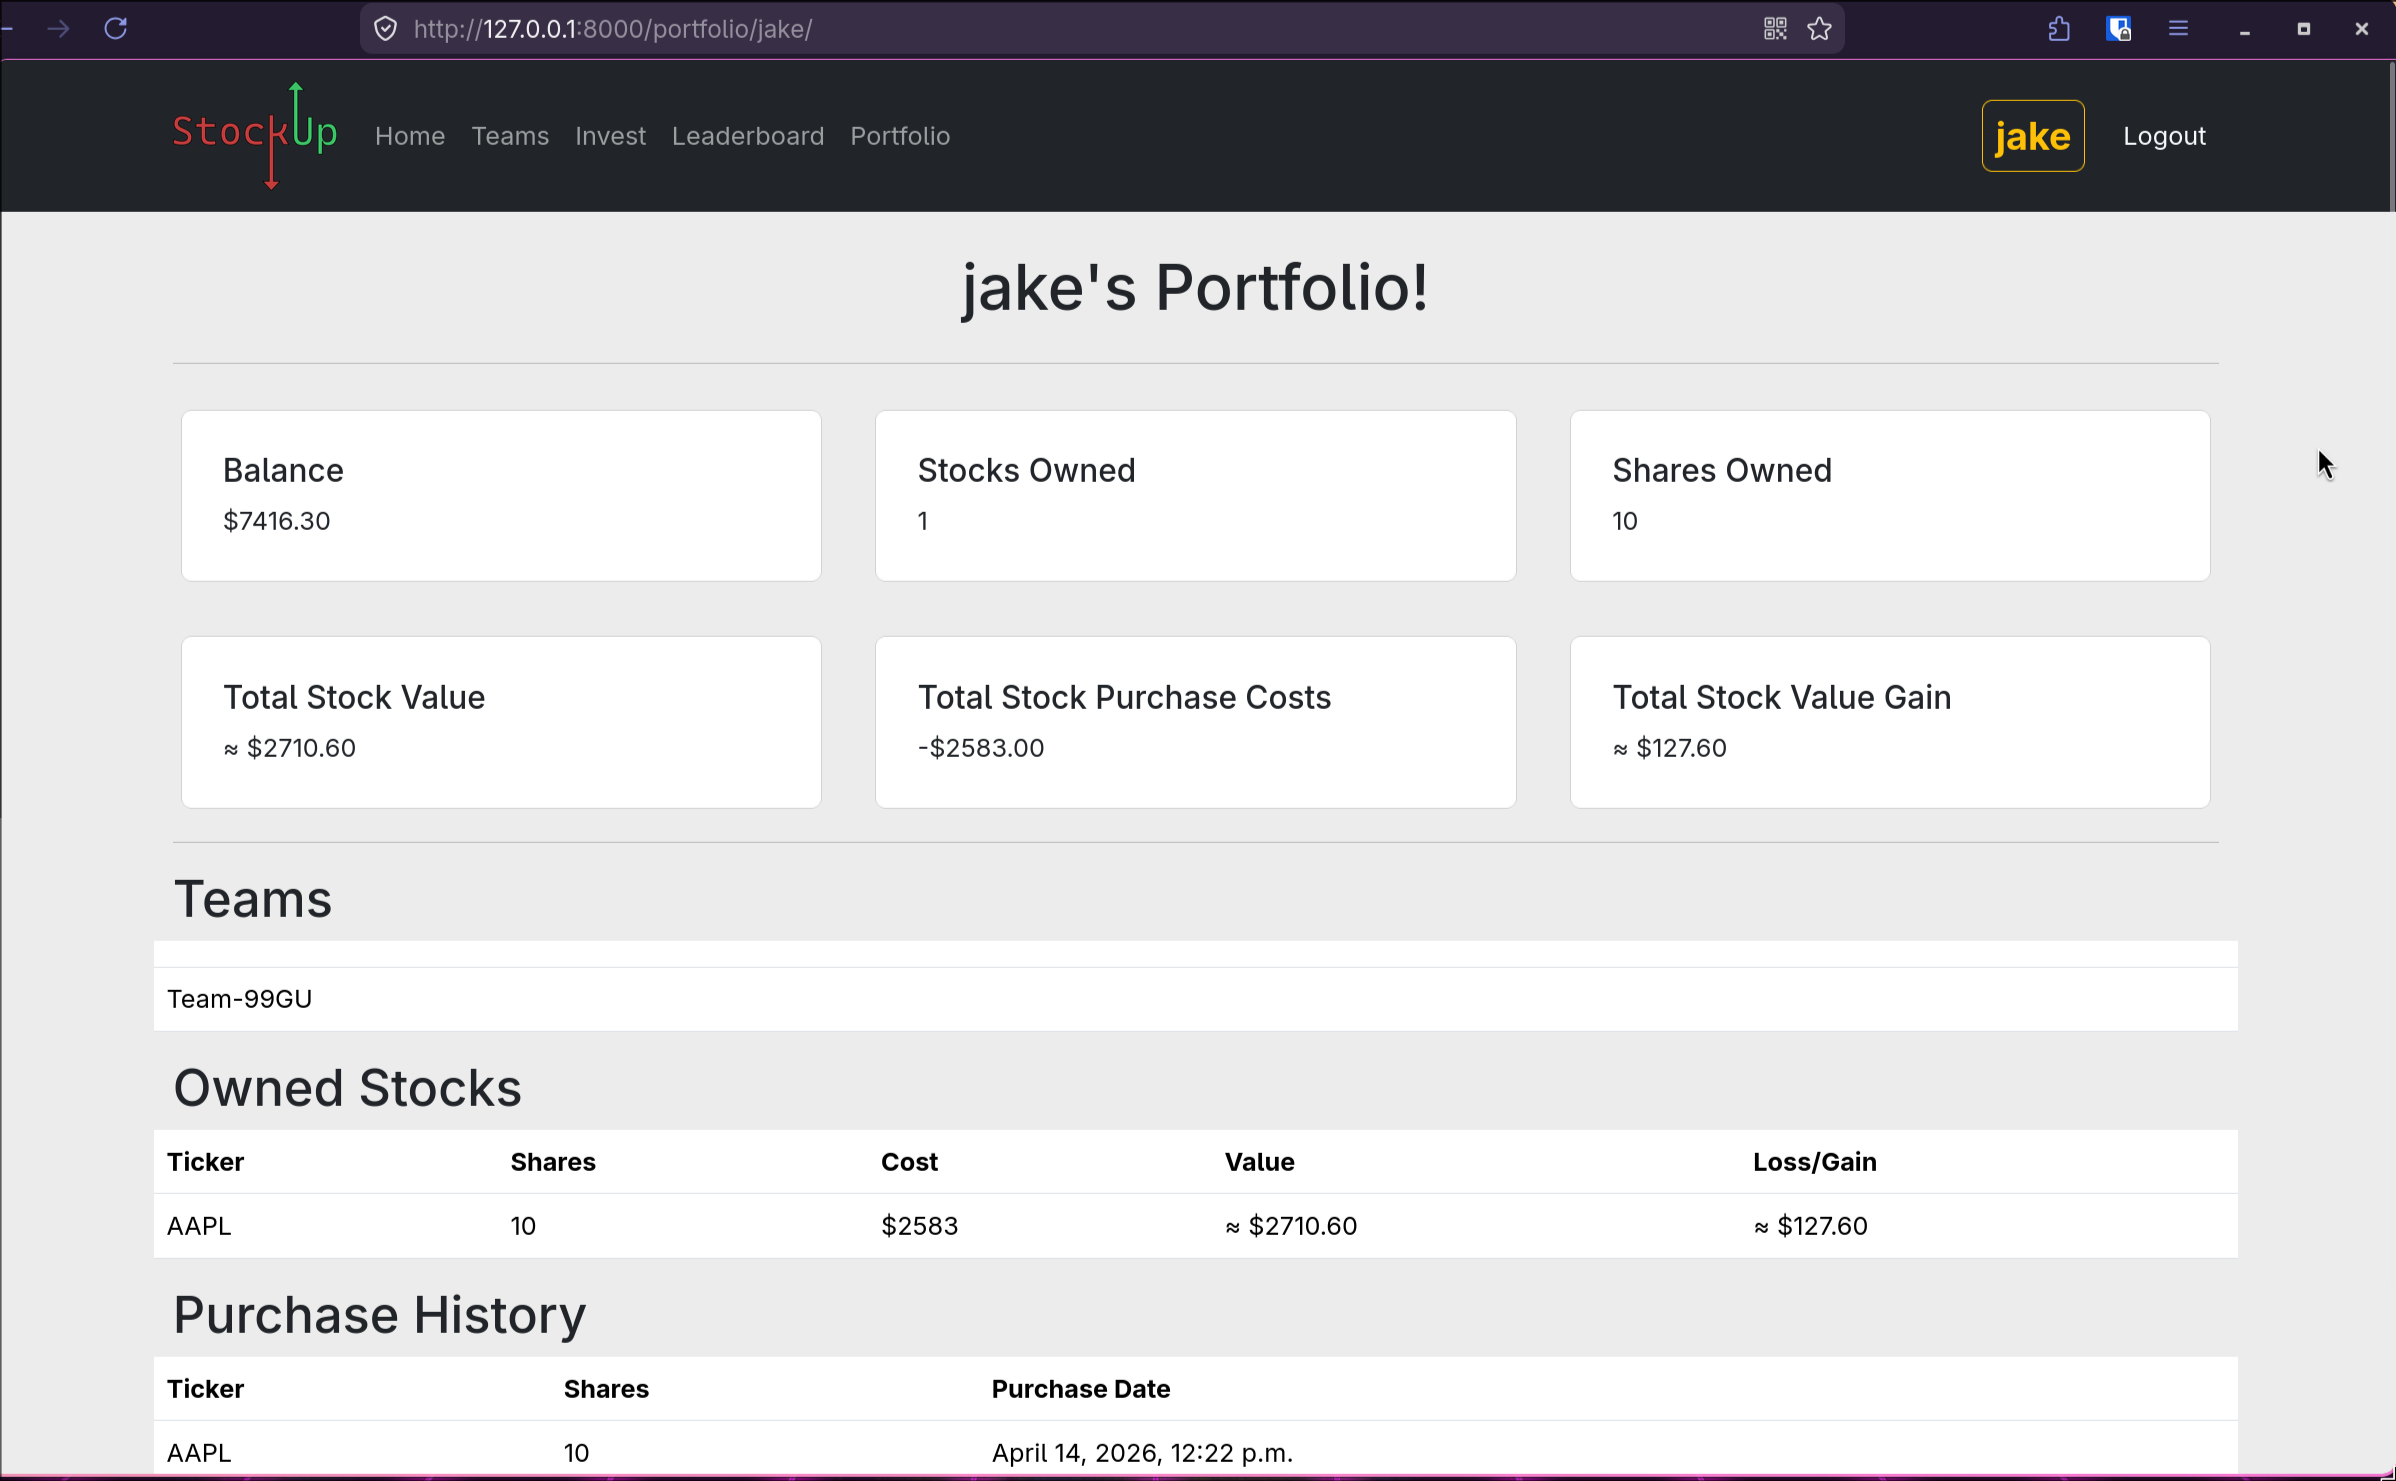
\includegraphics[width=0.7\linewidth]{portfolio.png}
        \caption{Portfolio Page}
        \label{fig:portfolio}
    \end{figure}
    
\section{Timeline of Deliverables}
    \begin{itemize}
        \item \textbf{April 15, 2026:} All parts of the project must work in isolation of each other. The website
        should be fully functional, the backend and API should be fully functional, and the database should be
        fully functional. At this point, the project should be done with Phase III.
        \item \textbf{May 1, 2026:} The project should be fully functional at this point. The required queries
        should be in place, and all aspects of the project should properly interact with minimal bugs. Phase IV
        should be complete at this point.
        \item \textbf{May 5, 2026:} The project must be complete by this point.
    \end{itemize}

    As of April 25, 2026, we are on track with our goal. Everything is functional, with just a handful of things left to add.
    The project will be ready for presentation by our set presentation date, which is May 5, 2026.
    
    \end{document}
    